\documentclass[12pt]{article}
\linespread{2}
\usepackage{times}
\usepackage{pgfplots}
\usepackage[dvipsnames]{xcolor}
\pgfplotsset{compat = newest}
\usetikzlibrary{positioning, arrows.meta}
\usepgfplotslibrary{fillbetween}
\usepackage{amsmath}
           \begin{document} 
                     \begin{center}
                          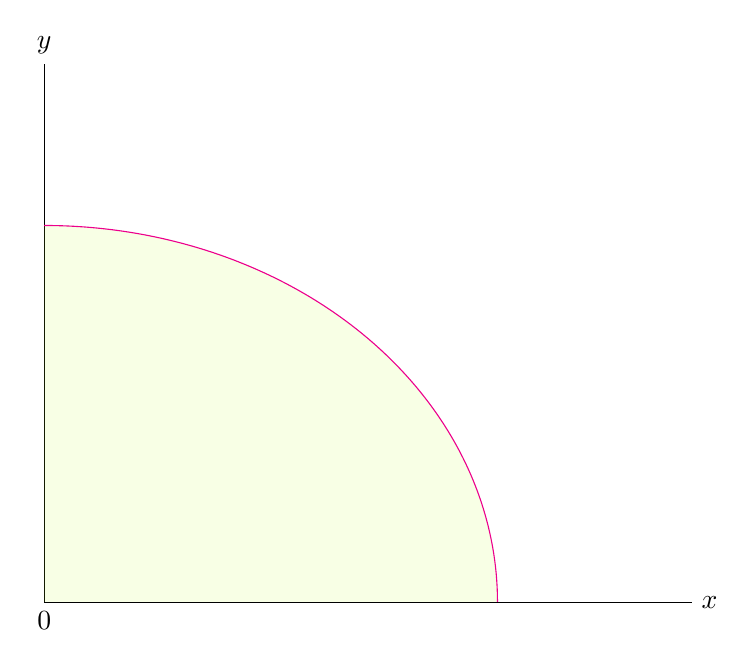
\begin{tikzpicture}
                                 \begin{axis}[
                                               scale = 1.2,
                                               xmin = 0, xmax = 10,
                                               ymin = 0, ymax = 10,
                                               axis lines* = left,
                                               xtick = {0}, ytick = \empty,
                                               clip = false,
]
% Production-possibility frontier
                        \addplot [domain = 0:10, restrict y to domain = 0:10, samples =
                                  10000, color = magenta, name path = frontier] {(49-x
                                  ^2)^0.5};
                        \addplot [domain = 0:10, restrict y to domain = 0:10, line width =
                                  0pt, name path = axis] {0};
                                              
% Colouring areas
                        \addplot [lime, draw = none, fill opacity = 0.1] fill between [of
                                  = frontier and axis];
                                  
% Labels
                        \node [right] at (current axis.right of origin){$x$};
                        \node [above] at (current axis.above origin) {$y$};
                       
                        
                     \end{axis}
               \end{tikzpicture}
       \end{center}

                \textbf{Figure 15 }
  \end{document} 